%==============================常用宏包、环境==============================%
\documentclass[twocolumn,a4]{article}
\usepackage{xeCJK} % For Chinese characters
\usepackage{amsmath, amsthm}
\usepackage{listings,xcolor}
\usepackage{geometry} % 设置页边距
\usepackage{fontspec}
\usepackage{graphicx}
\usepackage{float} %设置图片浮动位置的宏包
\usepackage{subfigure} %插入多图时用子图显示的宏包
\usepackage{fancyhdr} % 自定义页眉页脚
\setsansfont{Consolas} % 设置英文字体
\setmonofont[Mapping={}]{Consolas} % 英文引号之类的正常显示,相当于设置英文字体
\geometry{left=1cm,right=1cm,top=2cm,bottom=0.5cm} % 页边距
\setlength{\columnsep}{30pt}
% \setlength\columnseprule{0.4pt} % 分割线
%==============================常用宏包、环境==============================%

%==============================页眉、页脚、代码格式设置==============================%
% 页眉、页脚设置
\pagestyle{fancy}
% \lhead{CUMTB}
\lhead{\CJKfamily{hei} 泡泡猿专用模板}
\rhead{第 \thepage 页}
% \rhead{Page \thepage}
\chead{\leftmark} 
\lfoot{} 
\cfoot{}
\rfoot{}
\renewcommand{\headrulewidth}{0.4pt} 
\renewcommand{\footrulewidth}{0.4pt}

% 代码格式设置
\lstset{
    language    = c++,
    numbers     = left,
    numberstyle = \tiny,
    breaklines  = true,
    captionpos  = b,
    tabsize     = 4,
    frame       = shadowbox,
    columns     = fullflexible,
    commentstyle = \color[RGB]{0,128,0},
    keywordstyle = \color[RGB]{0,0,255},
    basicstyle   = \small\ttfamily,
    stringstyle  = \color[RGB]{148,0,209}\ttfamily,
    rulesepcolor = \color{red!20!green!20!blue!20},
    showstringspaces = false,
}
%==============================页眉、页脚、代码格式设置==============================%

%==============================标题和目录==============================%
\title{\CJKfamily{hei} \bfseries 泡泡猿ACM模板}
\author{Rand0w \& REXWIND \& Dallby}
\renewcommand{\today}{\number\year 年 \number\month 月 \number\day 日}

\begin{document}\small
\begin{titlepage}
\maketitle
\begin{figure}[H] %H为当前位置,!htb为忽略美学标准,htbp为浮动图形
\centering %图片居中
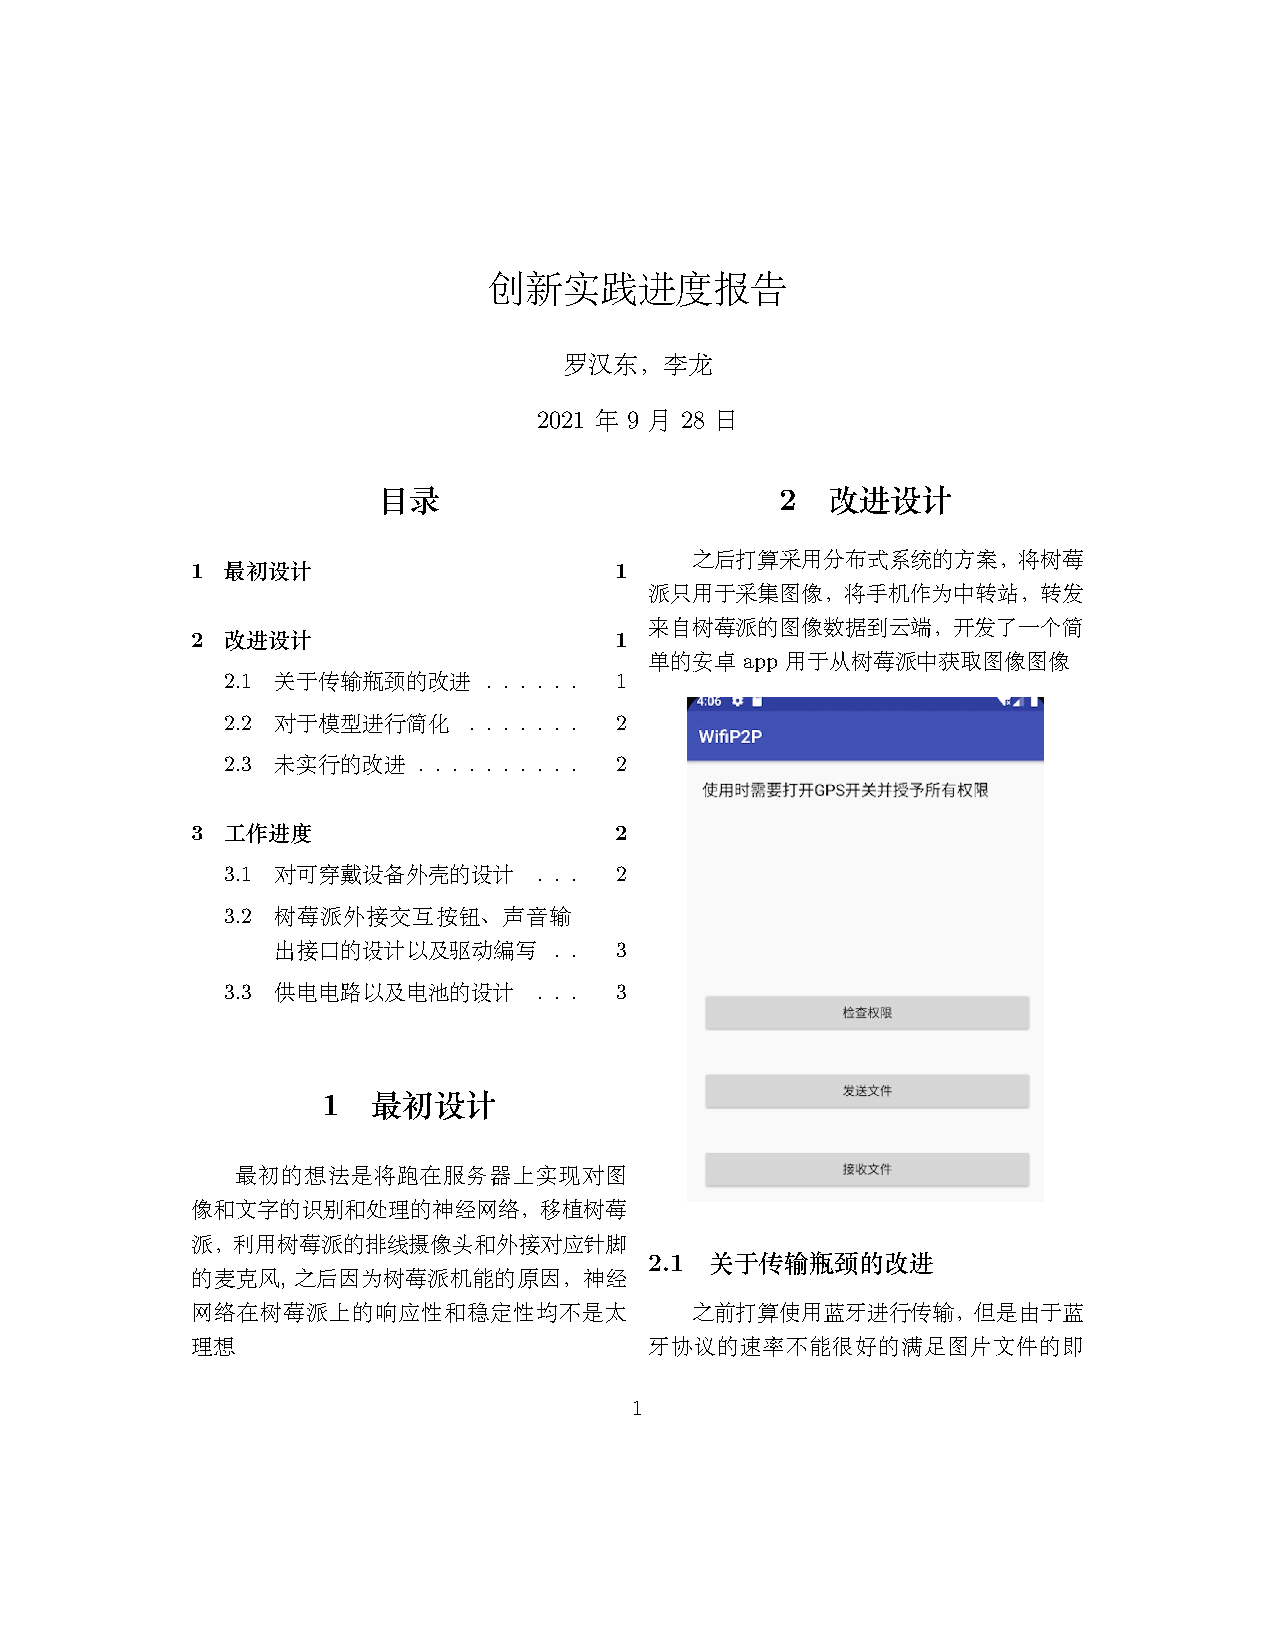
\includegraphics[width=0.7\textwidth]{1.jpg} %插入图片,[]中设置图片大小,{}中是图片文件名
\end{figure}
\end{titlepage}

\newpage
\pagestyle{empty}
\renewcommand{\contentsname}{目录}
\tableofcontents
\newpage\clearpage
\newpage
\pagestyle{fancy}
\setcounter{page}{1}   %new page
%==============================标题和目录==============================%

%==============================正文部分==============================%
\section{头文件}
\subsection{头文件(Rand0w)}
\begin{lstlisting}
#include <bits/stdc++.h>
//#include <bits/extc++.h>
//using namespace __gnu_pbds;
//using namespace __gnu_cxx;
using namespace std;
#pragma optimize(2)
//#pragma GCC optimize("Ofast,no-stack-protector")
//#pragma GCC target("sse,sse2,sse3,ssse3,sse4,popcnt,abm,mmx,avx,avx2,tune=native")
#define rbset(T) tree<T,null_type,less<T>,rb_tree_tag,tree_order_statistics_node_update>
const int inf = 0x7FFFFFFF;
typedef long long ll;
typedef double db;
typedef long double ld;
template<class T>inline void MAX(T &x,T y){if(y>x)x=y;}
template<class T>inline void MIN(T &x,T y){if(y<x)x=y;}
namespace FastIO
{
char buf[1 << 21], buf2[1 << 21], a[20], *p1 = buf, *p2 = buf, hh = '\n';
int p, p3 = -1;
void read() {}
void print() {}
inline int getc()
{
return p1 == p2 && (p2 = (p1 = buf) + fread(buf, 1, 1 << 21, stdin), p1 == p2) ? EOF : *p1++;
}
inline void flush()
{
fwrite(buf2, 1, p3 + 1, stdout), p3 = -1;
}
template <typename T, typename... T2>
inline void read(T &x, T2 &... oth)
{
int f = 0;x = 0;char ch = getc();
while (!isdigit(ch)){if (ch == '-')f = 1;ch = getc();}
while (isdigit(ch)){x = x * 10 + ch - 48;ch = getc();}
x = f ? -x : x;read(oth...);
}
template <typename T, typename... T2>
inline void print(T x, T2... oth)
{
if (p3 > 1 << 20)flush();
if (x < 0)buf2[++p3] = 45, x = -x;
do{a[++p] = x % 10 + 48;}while (x /= 10);
do{buf2[++p3] = a[p];}while (--p);
buf2[++p3] = hh;
print(oth...);
}
} // namespace FastIO
#define read FastIO::read
#define print FastIO::print
#define flush FastIO::flush
#define spt fixed<<setprecision
#define endll '\n'
#define mul(a,b,mod) (__int128)(a)*(b)%(mod) 
#define pii(a,b) pair<a,b>
#define pow powmod
#define X first
#define Y second
#define lowbit(x) (x&-x)
#define MP make_pair
#define pb push_back
#define pt putchar
#define yx_queue priority_queue
#define lson(pos) (pos<<1)
#define rson(pos) (pos<<1|1)
#define y1 code_by_Rand0w
#define yn A_muban_for_ACM
#define j1 it_is just_an_eastegg
#define lr hope_you_will_be_happy_to_see_this
#define int long long
#define rep(i, a, n) for (register int i = a; i <= n; ++i)
#define per(i, a, n) for (register int i = n; i >= a; --i)
const ll llinf = 4223372036854775851;
const ll mod = (0 ? 1000000007 : 998244353);
ll pow(ll a,ll b,ll md=mod) {ll res=1;a%=md; assert(b>=0); for(;b;b>>=1){if(b&1)res=mul(res,a,md);a=mul(a,a,md);}return res;}
const ll mod2 = 999998639;
const int m1 = 998244353;
const int m2 = 1000001011;
const int pr=233;
const double eps = 1e-7;
const int maxm= 1;
const int maxn = 510000;
void work()
{
	
}
signed main()
{
   #ifndef ONLINE_JUDGE
   //freopen("in.txt","r",stdin);
	//freopen("out.txt","w",stdout);
#endif
	//std::ios::sync_with_stdio(false);
	//cin.tie(NULL);
	int t = 1;
	//cin>>t;
	for(int i=1;i<=t;i++){
		//cout<<"Case #"<<i<<":"<<endll;
		work();
	}
	return 0;
}
\end{lstlisting}
\newpage
\subsection{头文件(REXWind)}
\begin{lstlisting}
#include<iostream>
#include<cstring>
#include<cstdio>
#include<algorithm>
#include<vector>
#include<map>
#include<queue>
#include<cmath>
using namespace std;

template<class T>inline void read(T &x){x=0;char o,f=1;while(o=getchar(),o<48)if(o==45)f=-f;do x=(x<<3)+(x<<1)+(o^48);while(o=getchar(),o>47);x*=f;}
int cansel_sync=(ios::sync_with_stdio(0),cin.tie(0),0);
#define ll long long
#define ull unsigned long long
#define rep(i,a,b) for(int i=(a);i<=(b);i++)
#define repb(i,a,b) for(int i=(a);i>=b;i--)
#define mkp make_pair
#define ft first
#define sd second
#define log(x) (31-__builtin_clz(x))
#define INF 0x3f3f3f3f
typedef pair<int,int> pii;
typedef pair<ll,ll> pll;
ll gcd(ll a,ll b){ while(b^=a^=b^=a%=b); return a; }
//#define INF 0x7fffffff

void solve(){
	
}

int main(){
	int z;
	cin>>z;
	while(z--) solve();
}
\end{lstlisting}
\subsection{头文件(Dallby)}
\begin{lstlisting}
#include<bits/stdc++.h>
cout<<"hello<<endl;
\end{lstlisting}
\section{数学}
\subsection{欧拉筛}
$O(n)$筛素数
\begin{lstlisting}
int primes[maxn+5],tail;
bool is_prime[maxn+5];
void euler()
{
   is_prime[1] = 1;
   for (int i = 2; i < maxn; i++)
   {
      if (!is_prime[i])
      primes[++tail]=i;
      for (int j = 0; j < primes.size() && i * primes[j] < maxn; j++)
      {
         is_prime[i * primes[j]] = 1;
         if ((i % primes[j]) == 0)
            break;
      }
   }
}
\end{lstlisting}
\subsection{Exgcd}
求出$ax+by=gcd(a,b)$的一组可行解 $O(logn)$ 
\begin{lstlisting}
void Exgcd(ll a,ll b,ll &d,ll &x,ll &y){
	if(!b){d=a;x=1;y=0;}
	else{Exgcd(b,a%b,d,y,x);y-=x*(a/b);}
}
\end{lstlisting}
\subsection{Excrt 扩展中国剩余定理}
求解同余方程组
$\begin{cases}
	\begin{aligned}
	x \ \% \ b_1  &\equiv \  a_1\\
	x \ \% \ b_2  &\equiv \ a_2\\
	           		& \ \vdots   \\
	x \ \% \ b_n  &\equiv  \ a_n
	\end{aligned}
\end{cases}$
\begin{lstlisting}
int excrt(int a[],int b[],int n)
{
    int lc=1;
    for(int i=1;i<=n;i++)
        lc=lcm(lc,a[i]);
    for(int i=1;i<n;i++){
        int p,q,g;
        g=exgcd(a[i],a[i+1],p,q);
        int k=(b[i+1]-b[i])/g;
        q=-q;p*=k;q*=k;
        b[i+1]=a[i]*p%lc+b[i];
        b[i+1]%=lc;
        a[i+1]=lcm(a[i],a[i+1]);
    }
    return (b[n]%lc+lc)%lc;
}
\end{lstlisting}
\subsection{线性筛逆元}
\begin{lstlisting}
void init(int p){
	inv[1] = 1;
	for(int i=2;i<=n;i++)
		inv[i] = (ll)(p-p/i)*inv[p%i]%p;
}
\end{lstlisting}
\subsection{计算一个数的$\varphi (x)$}
\begin{lstlisting}
int euler_phi(int n){
	int sqr = sqrt(n+0.5);
	int res = n; 
	for(int i=2;i<=sqr;i++){
		if(n%i==0){ 
			res = res/i*(i-1);
			while(n%i==0) n/=i;
		}
	}
	if(n>1) res = res/n*(n-1);
	return res; 
}
\end{lstlisting}
\subsection{Pollard\_Rho质因数分解}
\begin{lstlisting}
class ffj{
    public:
    ll tail;
    ll pp[1000];
    bool miller_rabin(ll a,ll n){
        ll d=n-1,r=0;
        while(!(d&1))d>>=1,r++;
        ll x=pow(a,d,n);
        if(x==1)return 1;
        for(int i=0;i<r;i++){
            if(x==n-1)return 1;
            x=mul(x,x,n);
        }
        return 0;
    }
    bool ttprime(ll x){
        if(x<=1)return 0;
        static int num[]={2,3,5,7,13,29,37,89};
        for(int i=0;i<8;i++)if(x==num[i])return 1;
        for(int i=0;i<8;i++)if(!miller_rabin(num[i],x))return 0;
        return 1;
    }
    ll fun(ll x,ll c,ll mod){
        return (mul(x,x,mod)+c)%mod;
    }
    ll gcd(ll n,ll m){
        if(m==0)return n;
        return gcd(m,n%m);
    }
    ll pollard_rho(ll x){
        ll c=rand()%(x-1)+1;
        ll s=0,t=0;
        for(int goal=1;;goal<<=1,s=t){
            ll val=1;
            for(int step=1;step<=goal;step++){
                t=fun(t,c,x);
                val=mul(val,abs(s-t),x);
                if(step%127==0){
                    ll d=gcd(val,x);
                    if(d>1)return d;
                }
            }
            ll d=gcd(val,x);
            if(d>1)return d;
        }
    }
    void find_fac(ll x){
        if(x==1)return;
        if(ttprime(x)){
            pp[++tail]=x;
            return;
        }
        ll y=x;
        while(y==x)y=pollard_rho(x);
        find_fac(y),find_fac(x/y);
    }
    void fj(ll x){
        tail=0;
        find_fac(x);
    }
}
\end{lstlisting}
\subsection{FFT快速傅里叶变换}
\begin{lstlisting}
const int SIZE=(1<<21)+5;
const double PI=acos(-1);
struct CP{
    double x,y;
    CP(double x=0,double y=0):x(x),y(y){}
    CP operator +(const CP &A)const{return CP(x+A.x,y+A.y);}
    CP operator -(const CP &A)const{return CP(x-A.x,y-A.y);}
    CP operator *(const CP &A)const{return CP(x*A.x-y*A.y,x*A.y+y*A.x);}
};
int limit,rev[SIZE];
void DFT(CP *F,int op){
    for(int i=0;i<limit;i++)if(i<rev[i])swap(F[i],F[rev[i]]);
    for(int mid=1;mid<limit;mid<<=1){
        CP wn(cos(PI/mid),op*sin(PI/mid));
        for(int len=mid<<1,k=0;k<limit;k+=len){
            CP w(1,0);
            for(int i=k;i<k+mid;i++){
                CP tmp=w*F[i+mid];
                F[i+mid]=F[i]-tmp;
                F[i]=F[i]+tmp;
                w=w*wn;
            }
        }
    }
    if(op==-1)for(int i=0;i<limit;i++)F[i].x/=limit;
}
void FFT(int n,int m,CP *F,CP *G){
    for(limit=1;limit<=n+m;limit<<=1);
    for(int i=0;i<limit;i++)rev[i]=(rev[i>>1]>>1)|((i&1)?limit>>1:0);
    DFT(F,1),DFT(G,1);
    for(int i=0;i<limit;i++)F[i]=F[i]*G[i];
    DFT(F,-1);
}
\end{lstlisting}
\subsection{NTT快速数论变换}
\begin{lstlisting}
const int SIZE=(1<<21)+5;
int limit,rev[SIZE];
void DFT(ll *f, int op) {
    const ll G = 3;
    for(int i=0; i<limit; ++i) if(i<rev[i]) swap(f[i],f[rev[i]]);
    for(int len=2; len<=limit; len<<=1) {
        ll w1=pow(pow(G,(mod-1)/len),~op?1:mod-2);
        for(int l=0, hf=len>>1; l<limit; l+=len) {
            ll w=1;
            for(int i=l; i<l+hf; ++i) {
                ll tp=w*f[i+hf]%mod;
                f[i+hf]=(f[i]-tp+mod)%mod;
                f[i]=(f[i]+tp)%mod;
                w=w*w1%mod;
            }
        }
    }
    if(op==-1) for(int i=0, inv=pow(limit,mod-2); i<limit; ++i) f[i]=f[i]*inv%mod;
}
void NTT(int n,int m,int *F,int *G){
    for(limit=1;limit<=n+m;limit<<=1);
    for(int i=0;i<limit;i++)rev[i]=(rev[i>>1]>>1)|((i&1)?limit>>1:0);
    DFT(F,1),DFT(G,1);
    for(int i=0;i<limit;i++)F[i]=F[i]*G[i];
    DFT(F,-1);
}
\end{lstlisting}
\subsection{MTT任意模数多项式乘法}
\begin{lstlisting}
struct MTT{
    static const int N=1<<20;
    struct cp{
        long double a,b;
        cp(){a=0,b=0;}
        cp(const long double &a,const long double &b):a(a),b(b){}
        cp operator+(const cp &t)const{return cp(a+t.a,b+t.b);}
        cp operator-(const cp &t)const{return cp(a-t.a,b-t.b);}
        cp operator*(const cp &t)const{return cp(a*t.a-b*t.b,a*t.b+b*t.a);}
        cp conj()const{return cp(a,-b);}
    };
    cp wn(int n,int f){
        static const long double pi=acos(-1.0);
        return cp(cos(pi/n),f*sin(pi/n));
    }
    int g[N];
    void dft(cp a[],int n,int f){
        for(int i=0;i<n;i++)if(i>g[i])swap(a[i],a[g[i]]);
        for(int i=1;i<n;i<<=1){
            cp w=wn(i,f);
            for(int j=0;j<n;j+=i<<1){
                cp e(1,0);
                for(int k=0;k<i;e=e*w,k++){
                    cp x=a[j+k],y=a[j+k+i]*e;
                    a[j+k]=x+y,a[j+k+i]=x-y;
                }
            }
        }
        if(f==-1){
            cp Inv(1.0/n,0);
            for(int i=0;i<n;i++)a[i]=a[i]*Inv;
        }
    }
    cp a[N],b[N],Aa[N],Ab[N],Ba[N],Bb[N];
    vector<ll> conv_mod(const vector<ll> &u,const vector<ll> &v,ll mod){ // 任意模数fft
        const int n=(int)u.size()-1,m=(int)v.size()-1,M=sqrt(mod)+1;
        const int k=32-__builtin_clz(n+m+1),s=1<<k;
        g[0]=0; for(int i=1;i<s;i++)g[i]=(g[i/2]/2)|((i&1)<<(k-1));
        for(int i=0;i<s;i++){
            a[i]=i<=n?cp(u[i]%mod%M,u[i]%mod/M):cp();
            b[i]=i<=m?cp(v[i]%mod%M,v[i]%mod/M):cp();
        }
        dft(a,s,1); dft(b,s,1);
        for(int i=0;i<s;i++){
            int j=(s-i)%s;
            cp t1=(a[i]+a[j].conj())*cp(0.5,0);
            cp t2=(a[i]-a[j].conj())*cp(0,-0.5);
            cp t3=(b[i]+b[j].conj())*cp(0.5,0);
            cp t4=(b[i]-b[j].conj())*cp(0,-0.5);
            Aa[i]=t1*t3,Ab[i]=t1*t4,Ba[i]=t2*t3,Bb[i]=t2*t4;
        }
        for(int i=0;i<s;i++){
            a[i]=Aa[i]+Ab[i]*cp(0,1);
            b[i]=Ba[i]+Bb[i]*cp(0,1);
        }
        dft(a,s,-1); dft(b,s,-1);
        vector<ll> ans;
        for(int i=0;i<n+m+1;i++){
            ll t1=llround(a[i].a)%mod;
            ll t2=llround(a[i].b)%mod;
            ll t3=llround(b[i].a)%mod;
            ll t4=llround(b[i].b)%mod;
            ans.push_back((t1+(t2+t3)*M%mod+t4*M*M)%mod);
        }
        return ans;
    }
}mtt;
\end{lstlisting}
%==============================正文部分==============================%
\end{document}